\documentclass[../main.tex]{subfiles}

\begin{document}


\section*{Appendix}  % Creates an unnumbered section called "Appendix"
\addcontentsline{toc}{section}{Appendix}
% Set subsections to be numbered as "A.1", "A.2", etc.
\renewcommand{\thesubsection}{A.\arabic{subsection}}  
\renewcommand{\thesection}{A}  % Set section label to "A" in the appendix
% Redefine theorem numbering for appendix with "A" prefix
\renewcommand{\thetheorem}{A.\thesection.\arabic{theorem}}
\setcounter{theorem}{0} % Reset theorem counter for the appendix
\newtheorem{appendixtheorem}{Theorem}[section] % Redefine with section-based numbering for appendix


\subsection{The Cause of the ``Strategic Effect''}
\label{sec:separate}

The main difference between our equilibrium and that of \cite{schnell2017physician} is the presence of a ``strategic effect'', wherein physician $j$ takes into account the behavior of other physicians in the selection of her own $\bar{\kappa_j}$. Of the different modifications we made to Schnell's framework, we argue that it is the absence of \textit{additive separability} across patients in physician utility $U_j(\cdot)$ which accounts for this.

In our context of unbounded maximization by physician $j$, the absence of additive separability implies she can't consider each patient individually when it comes to whether she's willing to allow (or induce) their visit, such a decision no longer being independent from other patients' visits in its impact to the physician's utility: the marginal utility of an additional patient is dependent on the aggregate of clients up to that point, both in terms of the visit itself as well as in the number of sick leaves granted up to that point.

Let's illustrate this point. Consider for a moment a finite number of patients $1, ... , k$, where each patient is inputed directly as an argument in our physician $j$'s utility function $U_j(\cdot)$, like so: $U_j(1, ..., k)$. If $U_j(\cdot)$ has the property of additive separability, this means it may be reformulated as the addition of individual functions for each patient:
\[
U_j(1, ...,k) = v_{j1}(1) + ... + v_{jk}(k) = \sum_{i = 1}^{k} v_{ji}(i)
\]
Unconstrained optimization in this context implies she's willing to see any patient whose $v_{ji}(i)$ is non-negative, such that her optimal level of utility is:
\[
U_j^*(1, ...,k) =  \sum_{i : \; v_{ji}(i) \geq 0} v_{ji}(i)
\]
For our physician-patient model, where physician utility is increasing in $\kappa_i$, such patient selection is achieved by the physician through the choice of $\kappa_j^*$, excluding all patients $i$ whose $\kappa_i < \kappa_j^*$. Supposing our patients are well-ordered in $\kappa_i$, the selection of such a $\kappa_j^*$ would be one where the marginal consumer $i$ affords a non-negative $v_{ji}(i)$, and the inframarginal consumer $i + 1$ satisfies $v_{j,i+1}(i+1) < 0$. Ignoring for a moment that patients themselves have a \textit{choice} of visiting—depending upon a second dimension $\gamma$ —, we would then have:
\[
U_j^*(1, ...,k) =  \sum_{i : \; \kappa_i \geq \kappa_j^*} v_{ji}(i)
\]

If instead of a discrete set we consider a mass of consumers $\mathcal{I}$ characterized by their level of $\kappa_i$, and we make the simplifying assumption that $v_{ji}$ takes on the same form $v_{j}$ for every $i \in \mathcal{I}$, our function $U_j(\cdot)$ could be expressed as:
\[
U_j^*(\mathcal{I}) =\int_{\kappa_j^*}^{\infty} v_{j}(\kappa) \, dF(\kappa)
\]

$U_j^*(\mathcal{I})$ represents the optimal value of $U_j(\mathcal{I})$, where physician $j$ only sees patients who provide her with non-negative marginal utility, i.e. such that $\kappa_i \geq \kappa_j^*$. We can find this optimal value $\kappa_j^*$ by looking at \textit{threshold} equilibria, where physician utility is also dependent on the threshold $\bar{\kappa_j}$ over which she's willing to see patients:
\[
U_j(\mathcal{I}, \bar{\kappa_j}) =\int_{\bar{\kappa_j}}^{\infty} v_{j}(\kappa) \, dF(\kappa)
\]

The optimal value of the threshold $\bar{\kappa_j}$ corresponds to that of $\kappa_j^*$. Assuming $U_j(\cdot) $ is twicely differentiable and concave in $\bar{\kappa_j}$, this solution may be arrived at through the FOC:
\[
\frac{\partial U_j(\mathcal{I})}{\partial \bar{\kappa_j}} \equiv - v_{j}(\bar{\kappa_j})f(\bar{\kappa_j}) = 0
\]
Solving for this would yield the optimal $\bar{\kappa_j} = \kappa_j^*$.

\cite{schnell2017physician} is an example of just such a treatment, which specifies the physician's additively separable utility by patient in the following manner:
\[
v_{ji}(\kappa_i) \equiv R_j + \beta_j h(\kappa_i)
\]
where $R_j$ is a parameter which stands for revenue by visit, and $\beta_j h(\kappa_i)$ represents the physician's `altruistic' utility over the health impact of a prescription drug to a patient with `pain level' $\kappa_i$.

The optimal threshold $\kappa_j^*$ is then obtained out of the maximization:\footnote{Once again, ignoring patient choice and $\gamma$,. We're discussing a \textit{simplified} version of the patient search framework for illustrative purposes.}
\[
\max_{\bar{\kappa_j}}\int_{\bar{\kappa_j}}^{\infty}  R_j + \beta_j h(\kappa) \, dF(\kappa)
\]

Resulting in the following FOC:
\[
R_j = - \beta_j h^{\prime}(\bar{\kappa_j})
\]
which, as is immediately apparent, doesn't depend upon the behavior of other physicians, more specifically, on \textit{their} choice of $\bar{\kappa_j}$. This equation merely establishes that, at the threshold, marginal benefit by patient—revenue $R_j$—must equal marginal ``cost'', the altruistic ``cost'' $\beta_j h(\bar{\kappa_j})$. A way to interpret this is that physicians will be willing to see any patient which render them positive marginal utility, unconcerned with their total market share, and thus, unconcerned with what other physicians may do to take away clientele.

A treatment like Schnell's is rendered inviable by our choice of utility function. Her parameter of revenue would in our model imply the linearity of our revenue \textit{function} $R_j(\cdot)$ and our $P(\cdot)$ function over \textit{aggregate} licenses granted. Strict convexity of $P(\cdot)$ would forestall its formulation as Schnell-like $\beta_j h^{\prime}(\bar{\kappa_j})$ terms for each patient, because the impact on doctor $j$'s utility in granting patient $i$ a license would no longer independent from the granting of licenses of other patients. Likewise, strict concavity of $R_j(\cdot)$ belies a simple ``r'' parameter such that $R_j'(Q_j) = r Q_j$.

More formally, when $U_j(1,...,k)$ \textit{isn't} additively separable across patients, the value $\kappa_j^*$ such that if $\kappa_i \geq \kappa_j^*$ patient $i$ provides positive marginal utility, isn’t independent of current clientele, because what before was a properly defined object, marginal utility by patient $i$, $v_j(\kappa_i)$, can no longer be so identified. The marginal utility $i$ provides to $j$ as the $k$th client (assuming some order over clients) is not necessarily the same he’d provide as the $k+1$th client, and so, as the $k$th client he could provide $0$ utility, impliying $\kappa_i = \kappa_j^*$, whereas as the $k + 1$th he could be inframarginal, such that $\kappa_i < \kappa_j^*$.

$\kappa_j^*$ is not longer independent of clientele mass $\mathcal{I}$ as before, but a function of it, $\kappa_j^*(\mathcal{I})$. More specifically, in the models we consider it will depend on the \textit{cardinality} of current clientele, $|\mathcal{I}|$, such that our physician's choice of marginal consumer will depend on her aggregate level of patient demand, where before it didn't. This effect is introduced through the \textit{strict non-linearity} of our physician utility function $U_j(\cdot)$, either through the strict concavity of $R_j(\cdot)$ over expected patient demand $Q_j$, or the strict convexity of $P_j(\cdot)$ over total expected sick leaves granted.

When either of those is the case, $aggregate$ levels enter into the equation and form part of the optimality condition. Our general FOC reflects this:
\begin{equation}
 R_j^{\prime}(Q_j)\frac{\partial Q_j}{\partial\bar{\kappa_j}} = P_j^{\prime}(X_j)\frac{\partial X_j}{\partial \bar{\kappa_j}} 
 \label{eq:apx_foc}
\end{equation}
where either or both of $R_j'(\cdot)$ and $P_j'(\cdot)$ are a non-constant function over aggregates.

When such aggregates, either $Q_j$ or $X_j$, come into play, physicians come to consider their \textit{market share}, which doesn't depend exclusively on their own choice of $\bar{\kappa_j}$. Each patient's strategy $S_i$ is constructed taking into account the whole of $\{(V_j,\bar{\kappa_j})\}_{i =1}^{J}$.

Imagine equation (\ref{eq:apx_foc}) holds for some doctor $j$, and some doctor $l \neq j$ decides to lower her $\bar{\kappa_l}$, enough that it changes the value of $s_{ij}$ for some mass of clients. The value of $Q_j$ would then change, and therefore that of $ R_j^{\prime}(Q_j)$. If $P_j^{\prime}(X_j)$ didn't vary by the same amount, (\ref{eq:apx_foc}) would no longer be an equality, leading $j$ to modify her choice of $\bar{\kappa_j}$ to make equality hold.

This intelligible line of reasoning links the presence of a ``strategic effect'' to the non-additive separability of $U_j(\cdot)$: doctor $j$ takes into account other physicians' strategy in her own choice of $ \bar{\kappa_j}$ because of the present of \textit{aggregate} amounts of clientele in her optimality conditions, which is so because utility isn't additively separable across clients.

\subsection{\cite{schnell2017physician} with Logit Choice}
\label{sec:schnell_logit}

To prove our point that it is additive separability which accounts for a possible strategic effect, we reformulate \cite{schnell2017physician} in the manner of a McFadden Logit — with some quirks.

The way in which Schnell devises her physician's utility formula is implicitly Bernoulli-like:
\[
\int_{\kappa} \int_{\gamma} u(\kappa, \gamma) \cdot p(\kappa, \gamma) \, dG(\gamma) dF(\kappa)
\]
where $u(\kappa, \gamma)$ is the utility function of the physician from patients characterized by a given $(\kappa, \gamma)$ tuple, and $p(\kappa, \gamma)$ stands for the density of clients atomized in this tuple.

We define $u(\kappa, \gamma)$ as Schnell did: $\beta_j h(\kappa) + R_j$. The accompanying $p(\kappa, \gamma)$ fits the role that our own $s_{ij}$ we have been playing thus far, which implicitly depends on the $(\kappa_i, \gamma_i)$ tuple which characterizes patient $i$, and gives a measure of the change that they'll visit physician $j$. Physician utility can thus be rendered as:
\[
\int_{\kappa} \int_{\gamma} [\beta_j h(\kappa) + R_j] \cdot s_{ij}(\kappa, \gamma) \, dG(\gamma) dF(\kappa)
\]


In our modeling section, our ``implicit'' search model was a left-censored Logit choice model, which gave null probability of assignment to physicians from which patient $i$ expected non-positive utility. It was defined as:
\[
s_{ij} = \frac{\alpha_{ij}}{\sum_{k = 1}^{J} \alpha_{ik}}, \; \; \text{where } \; \alpha_{ij} = \begin{cases}
e^{\lambda u_{ij}}, \; \; \text{if } \; \; u_{ij} > 0 \\
0 , \; \; \text{if } \; \; u_{ij} = 0
\end{cases}
\]

Schnell's opioid-focused physician model provides an additional simplification: patients which aren't given a drug prescription, i.e. those such that $\kappa_i < \bar{\kappa_j}$, don't garner positive utility from a visit. As such, in the original model as in this reformulation, patients ``below'' $\bar{\kappa_j}$ have a null probability of visit, making the lower bound of integration for $\kappa$ to be $\bar{\kappa_j}$.

As for $\gamma$, the lower bound of the inner integral remains the same as in Schnell in the absence of a secondary market, a value of $\gamma_i$ such that $u_{ij} = 0$, i.e. $h(\kappa_i) + \gamma_i - \tau^d - \tau^o = 0$.\footnote{Schnell splits the costs a patient will face into costs of visit ($\tau^d$), cost of purchase ($\tau^o$) and search cost ($\tau^s$), whereas we consider only the first.}

The double-integral of physician utility to be maximized is then as follows:
\[
\max_{\bar{\kappa_j}}\int_{\bar{\kappa_j}}^{\infty} \int_{\tau^d - \tau^o - h(\kappa)}^{\infty} [\beta_j h(\kappa) + R_j] \cdot \frac{e^{\lambda u_{ij}}}{\sum \limits_{k : \, u_{ik} > 0} e^{\lambda u_{ik}}} \, dG(\gamma) dF(\kappa)
\]

The FOC of this equation is:
\begin{equation}
    \underbrace{[\beta_j h(\bar{\kappa_j}) + R_j]}_{A}\underbrace{\int_{\tau^d - \tau^o - h(\bar{\kappa_j})}^{\infty} \frac{e^{\lambda u_{ij}} \mid \bar{\kappa_j}}{\sum \limits_{k : \, u_{ik} > 0} e^{\lambda u_{ik}} \mid \bar{\kappa_j}} \, dG(\gamma)}_{B} \underbrace{f(\bar{\kappa_j})}_{C} = 0 
\label{eq:schnell_logit}
\end{equation}
where we use ``$\mid \bar{\kappa_j}$'' to clumsily indicate that we integrate $\gamma$ over patients where $\kappa_i = \bar{\kappa_j}$. As an integral over a strictly positive value and the atom of a density function, respectively, the factors B and C in the equation are non-negative. For this reason, the only way for equation (\ref{eq:schnell_logit}) to be satisfied is by obeying the following equality:
\begin{equation}
    R_j = - \beta_j h(\bar{\kappa_j})
    \label{eq:schnell_condition}
\end{equation}

This is the same result as in the baseline model presented in \cite{schnell2017physician}, without a secondary market. This equality requires that marginal utility in $\bar{\kappa_j}$ must be $0$, i.e. that revenue ($R_j$) must equal "altruistic" loss ($\beta_j h(\bar{\kappa_j})$), which presupposes that the marginal patient granted prescription opioids suffers a net loss in utility (the negative externalities outweigh its medical benefit as a palliative).

Equation (\ref{eq:schnell_condition}) also implies that the value of  $\kappa_j$ is chosen with no considerarion of the strategies employed by other physicians, they quite literally don't enter into the equation. As we have argued, additive separability over clients means the \textit{aggregate} demand for physician $j$'s services doesn't influence marginal utility by a single patient $i$, and so it has no sway in the optimality condition. Physician $j$ follows simply the rule that she won't grant a prescription (or sick leave, as in our case) below $\bar{\kappa_j}$, however that might affect the size of her ``clientele''. In order for her to care about \textit{aggregate} values, like her total expected demand, making her take her market share and thus the strategies of other doctors into account, \textit{strict non-linearity} must be introduced into her utility function, either through $R_j(\cdot)$ or, as in our case, a function $P(\cdot)$.


\subsection{Strategic Complementarity of $\bar{\kappa_j}$'s (Proof of Proposition \ref{complements})}
\label{sec:strategic}

We defined the components $s_{ij}$ of $S_i$  as:
\[s_{ij} \equiv g_i(u_{ij}, u_{i,-j})\]
where $g_i(\cdot)$ is a continuous function weakly increasing in the first argument $u_{ij}$, weakly decreasing in $u_{i,-j}$. Our defining $s_{ij}$ this way has two interlinked corollaries:

\begin{corollary}
\[s_{ij} \mid \kappa_i < \bar{\kappa_j} \;\;\;\; \leq     \;\;\;\; s_{ij} \mid \kappa_i \geq \bar{\kappa_j} \;\;\;\; \text{(with strict inequality if $\gamma_i > 0$).}\]
\end{corollary}

\begin{proof}
    For a fixed value of $V_j$ and $\kappa_i$, for all $i$, the value of $U_i(V_j, \bar{\kappa_j})$ is $V_j \kappa_i - \tau_j$ if $\kappa_i < \bar{\kappa_j}$, and $\gamma_i + V_j \kappa_i - \tau_j$ if $\kappa_i \geq \bar{\kappa_j}$, where $\gamma_i \geq 0$. Given that $s_{ij}$ is weakly increasing in $u_{ij}$, and we see that $u_{ij}$ is weakly higher if $\kappa_i \geq \bar{\kappa_j}$, the corollary follows.
\end{proof}


\begin{corollary}
\begin{align*}
    \frac{\Delta s_{ij}}{\Delta\bar{\kappa_{j}}} \leq 0 &&  \frac{\Delta s_{ij}}{\Delta\bar{\kappa_{l}}} \geq 0, \forall l \neq j
\end{align*}   
\end{corollary}

\begin{proof}
From the argumentation in corollary 1 follows that $u_{ij}$ is weakly decreasing in $\bar{\kappa_j}$, $\forall j$. Take some $l \neq j$, then $s_{ij}$ is defined in turn as weakly decreasing in $u_{il}$, which implies it is increasing in $\bar{\kappa_l}$.
\end{proof}

Both corollaries hinge upon our definition of $U_i(\cdot)$ as a step function over $\kappa_i$, such that it is discontinuous at $\kappa_i = \bar{\kappa_j}$, where there's a discrete jump of magnitude  $\gamma_i \geq 0$. We use them in the next proposition.

\begin{prop}
\begin{align*}
    \frac{\partial Q_{j}}{\partial\bar{\kappa_{j}}},\frac{\partial X_{j}}{\partial\bar{\kappa_{j}}} \leq 0 &&  \frac{\partial Q_{j}}{\partial\bar{\kappa_{l}}}, \frac{\partial X_{j}}{\partial\bar{\kappa_{l}}} \geq 0, \forall l \neq j
\end{align*}
\end{prop}

\begin{proof}
We recall our function of patient demand for physician $j$ is:
    \[
    Q_j(\bar{\kappa_j}, \bar{\kappa}_{-j}) \,=\, \int_{0}^{\infty} \int_{0}^{\infty} s_{ij} (\kappa, \gamma) \,dG(\gamma) \,dF(\kappa) 
    \]
Were physician $j$ to increase her threshold from $\bar{\kappa_j}$ to $\bar{\kappa_j}' = \bar{\kappa_j} + \epsilon, \epsilon > 0$, for the mass of patients whose $\kappa_i \in [\bar{\kappa_j}, \bar{\kappa_j} + \epsilon)$, utility would weakly decrease and thus so would their $s_{ij}$, falling to ${s_{ij}}^{\prime} \leq s_{ij}$ (see first corollary, think of ${s_{ij}}^{\prime}$ as $s_{ij} \mid \kappa_i < \bar{\kappa_j}$ as opposed to $s_{ij} \mid \kappa_i \geq \bar{\kappa_j}$).

The difference that would make for patient demand \textit{caeteris paribus} given the $\bar{\kappa}_{-j}$ strategies of the other physicians (ommitted in our notation) is:\footnote{Besides simplifying $Q_j(\bar{\kappa_j}, \bar{\kappa}_{-j})$ into $Q_j(\bar{\kappa_j})$, we also forego the arguments of $s_{ij} (k, \gamma)$, as we've done many times already, to avoid notation clutter. }
\[
\Delta Q_j = Q_j(\bar{\kappa_j} + \epsilon) - Q_j(\bar{\kappa_j})=\int_{\bar{\kappa_j}}^{\bar{\kappa_j} + \epsilon} \int_{0}^{\infty} \{ {s_{ij}}^{\prime} - s_{ij}\} \,dG(\gamma) \,dF(\kappa)
\]

By the definition of a partial derivative:\footnote{The notation for ${s_{ij}} (\bar{\kappa_j}, \gamma)^{\prime}$ is to be taken to mean the strategy ${s_{ij}}^{\prime} \leq s_{ij}$ of the mass of patients at different levels of $\gamma$ atomized at $\kappa_i = \bar{\kappa_j}$.}
\begin{align*}
    \frac{\partial Q_{j}}{\partial\bar{\kappa_{j}}} & = \lim_{\epsilon \rightarrow 0} \frac{\int_{\bar{\kappa_j}}^{\bar{\kappa_j} + \epsilon} \int_{0}^{\infty} \{ {s_{ij}}^{\prime} - s_{ij}\} \,dG(\gamma) \,dF(\kappa)}{\epsilon} \\
    & = \int_{0}^{\infty} \{ {s_{ij}} (\bar{\kappa_j}, \gamma)^{\prime} - s_{ij} (\bar{\kappa_j}, \gamma)\} \,dG(\gamma) \,f(\bar{\kappa_j}) 
\end{align*}
where the derivative is negative if ${s_{ij}}^{\prime}$ is strictly lower than $s_{ij}$, meaning a shift in leniency would affect the utility and optimal strategy of some positive mass of patients around $\bar{\kappa_j}$; or null, if ${s_{ij}}^{\prime} = s_{ij}$.

In a similar vein, consider some physician $l \neq j$ shifting her threshold from $\bar{\kappa_{l}}$ to $\bar{\kappa_l}' = \bar{\kappa_l} + \epsilon, \epsilon > 0$. The fall in patient strategies in $[\bar{\kappa_j}, \bar{\kappa_j} + \epsilon)$ from $s_{il}$ to ${s_{il}}^{\star} \leq s_{il}$ could provide a windfall for $j$ (and all other physicians), raising $s_{ij}$ to ${s_{ij}}^{\star} \geq s_{ij}$ (see previous corollary). In that case:
\[
\Delta Q_j = \int_{\bar{\kappa_l}}^{\bar{\kappa_l} + \epsilon} \int_{0}^{\infty} \{ {s_{ij}}^{\star} - s_{ij}\} \,dG(\gamma) \,dF(\kappa) 
\]
thus rendering:
\begin{align*}
    \frac{\partial Q_{j}}{\partial\bar{\kappa_{l}}} & = \lim_{\epsilon \rightarrow 0} \frac{\int_{\bar{\kappa_l}}^{\bar{\kappa_l} + \epsilon} \int_{0}^{\infty} \{ {s_{ij}}^{\prime} - s_{ij}\} \,dG(\gamma) \,dF(k)}{\epsilon} \\
    & = \int_{0}^{\infty} \{ {s_{ij}} (\bar{\kappa_l}, \gamma)^{\star} - s_{ij} (\bar{\kappa_l}, \gamma)\} \,dG(\gamma) \,f(\bar{\kappa_l}) 
\end{align*}

As for $X_j$, the steps taken are almost the same, only that after raising the threshold by $\epsilon$ the amount of sick leaves granted goes around $\bar{\kappa_j}$ goes to $0$, thus giving out:
\[
\frac{\partial X_{j}}{\partial\bar{\kappa_{j}}} = - \int_{0}^{\infty}  s_{ij} (\bar{\kappa_j}, \gamma) \,dG(\gamma) \,f(\bar{\kappa_j})
\]
such that it is simply required that $j$ has positive demand for the mass of patients whose $\kappa_i = \bar{\kappa_j}$ for this derivative to be strictly negative, else it is null.

Likewise:
\[
\frac{\partial X_{j}}{\partial\bar{\kappa_{l}}} = - \int_{0}^{\infty}  s_{ij} (\bar{\kappa_l}, \gamma) \,dG(\gamma) \,f(\bar{\kappa_l})
\]

\end{proof}

Before dealing with Proposition \ref{complements} we need one last intermediary proposition.

\begin{prop}
\[
\frac{\partial^2 Q_{j}}{\partial\bar{\kappa_{j}} \partial\bar{\kappa_{l}}} = 0 \;\;\; \text{ and } \;\;\; \frac{\partial^2 X_{j}}{\partial\bar{\kappa_{j}} \partial\bar{\kappa_{l}}} = 0 \;, \;\;\; \text{ $\forall j$ and $l$, $\bar{\kappa_{j}} \neq \bar{\kappa_{l}}$}
\]
 \end{prop}

\begin{proof}
Our proof will be heuristic. Consider
 \[
    \frac{\partial Q_{j}}{\partial\bar{\kappa_{j}}} = \int_{0}^{\infty} \{ {s_{ij}} (\bar{\kappa_j}, \gamma)^{\prime} - s_{ij} (\bar{\kappa_j}, \gamma)\} \,dG(\gamma) \,f(\bar{\kappa_j})
 \]

Patient strategies $s_{ij}$ are taken at the atom $\kappa_i = \bar{\kappa_j}$. For any other physician $l$ such that $\bar{\kappa_l} \neq \bar{\kappa_j}$, an infinitesimally small change to $\bar{\kappa_l}$ doesn't affect the utility of patients at $\bar{\kappa_j}$, who will remain above or below $l$'s threshold same as before. Thus their strategy $s_{ij}$ also remains unaffected. If $\bar{\kappa_l}$ \textit{does} equal $\bar{\kappa_j}$, then the following limit is not properly defined:
\[
    \lim_{\epsilon \rightarrow 0} \frac{ \frac{\partial Q_{j}(\kappa_l + \epsilon)}{\partial\bar{\kappa_{j}}} - \frac{\partial Q_{j}(\kappa_l ) }{\partial\bar{\kappa_{j}}}   }{\epsilon}
\]
because as $\epsilon$ approaches $0$ from the right the limit is weakly positive ($\geq 0$), whereas approaching from the left it's strictly $0$. Meaning the derivative $\frac{\partial^2 Q_{j}}{\partial\bar{\kappa_{j}} \partial\bar{\kappa_{l}}}$ doesn't exist for $j$ and $l \neq j$ when $\bar{\kappa_j}=\bar{\kappa_l}$.

\end{proof}

\textit{Proof of Proposition \ref{complements}.}

Consider some two physicians $j$, $l$, such that $\bar{\kappa_j} \neq \bar{\kappa_l}$. If we breakdown the mixed partial derivative of $U_j$ over $\bar{\kappa_j}$ and $\bar{\kappa_l}$, we get:
\begin{align*}
\frac{\partial^2 U_{j}}{\partial\bar{\kappa_{j}} \partial\bar{\kappa_{l}}} = & 
\underbrace{R_j^{\prime \prime}(Q_j(\bar{\kappa_j}, \bar{\kappa}_{-j}))}_{\leq 0}
\cdot \underbrace{\frac{\partial Q_{j}}{\partial\bar{\kappa_{l}}}}_{\geq 0}
\cdot \underbrace{\frac{\partial Q_{j}}{\partial\bar{\kappa_{j}}}}_{\leq 0}  + 
\underbrace{R_j^{\prime} (Q_j(\bar{\kappa_j}, \bar{\kappa}_{-j}))}_{\geq 0} \underbrace{\frac{\partial^2 Q_{j}}{{\partial\bar{\kappa_{j}} \partial\bar{\kappa_{l}}}}}_{= \, 0} & \\
 & - \underbrace{P^{\prime \prime} (X_j(\bar{\kappa_j}, \bar{\kappa}_{-j}))}_{\geq 0}
\cdot \underbrace{\frac{\partial X_{j}}{\partial\bar{\kappa_{l}}}}_{\geq 0}
\cdot \underbrace{\frac{\partial X_{j}}{\partial\bar{\kappa_{j}}}}_{\leq 0}  - 
\underbrace{P^{\prime} (X_j(\bar{\kappa_j}, \bar{\kappa}_{-j}))}_{\geq 0} \underbrace{\frac{\partial^2 X_{j}}{\partial\bar{\kappa_{j}} \partial\bar{\kappa_{l}}}}_{= \, 0} &  \\
    = & \, \underbrace{{R_j^{\prime \prime}} (Q_j(\bar{\kappa_j}, \bar{\kappa}_{-j}))
    \cdot \frac{\partial Q_{j}}{\partial\bar{\kappa_{l}}}
    \cdot \frac{\partial Q_{j}}{\partial\bar{\kappa_{j}}}}_{\geq 0}  -
    \underbrace{P^{\prime \prime} (X_j(\bar{\kappa_j}, \bar{\kappa}_{-j}))
    \cdot \frac{\partial X_{j}}{\partial\bar{\kappa_{l}}}
    \cdot \frac{\partial X_{j}}{\partial\bar{\kappa_{j}}}}_{\leq 0} \, & \geq 0
\end{align*}
and positive mixed derivative of physicians' utility over their strategy is the definition of strategic complementarity.
\begin{flushright}
    $\square$
\end{flushright}

\subsection{Optimal Reserve Utility (Proof of Equation \ref{eq:seq4})}
\label{sec:sequential}

We follow the argument of \cite{sargent}. Let for the moment $\tilde{F_i}(U) = \operatorname{Pr}\{u_{ij} \leq U\}$ be the distribution of utility patient $i$ recieves from doctor visits, with $\tilde{F_i}(0) = 0$, $\tilde{F_i}(B) = 1$, for $B < \infty$. Each period, the patient draws an `offer' $U$ from $\tilde{F_i}$, which is to say, his search lead him to a physician $j$ such that $u_{ij} = U$. He may either accept and have physician $j$ assigned to him, recieving utility $U$ per period henceforth, or look for a new physician next period.

Let $u_t$ be the patient's utility for period $t$, where it's $0$ if he doesn't visit a physician and $U$ if he has accepted an assigned physician which renders him utility $u_{ij} = U$. This patient will seek to maximize $\mathbb{E}[\sum_{t=0}^{\infty} \beta^t u_t]$, where $0 < \beta < 1$ is his discount factor.

Let $V(U)$ be the expected value of $\sum_{t=0}^{\infty} \beta^t u_t$ of a patient with an offer $U$ in hand. Assuming no recall, under optimal behavior the value function $V(U)$ satisfies the Bellman equation:
\begin{equation}
    V(U) = \max \left\{ \frac{U}{1 - \beta},\; \;\beta \hspace{-0.1cm}\int V(U') \, d \tilde{F_i}(U') \right\}
    \label{eq:seq1} 
\end{equation}

The patient chooses an optimal value $\bar{U_i}$, such that offers $U \geq \bar{U_i}$ are accepted (the visit takes place). As such, the solution takes on the following form:
\begin{equation}
    V(U) = \begin{cases}
        \frac{\bar{U}_i}{1 - \beta} + \beta \int V(U') \, d \tilde{F_i}(U') & \text{if }\; \; U \leq \bar{U}_i, \\[0.5em]
        \frac{U}{1 - \beta} & \text{if } \; \; U \geq \bar{U}_i.
    \end{cases}
\label{eq:seq2} 
\end{equation}

Using equation (\ref{eq:seq2}), we can convert the functional equation (\ref{eq:seq1}) into an ordinary equation in the reservation utility $\bar{U_i}$. Evaluating $V(\bar{U_i})$ and using equation (\ref{eq:seq2}), we have:
$$
\frac{\bar{U_i}}{1-\beta}= \beta \int_0^{\bar{U_i}} \frac{\bar{U_i}}{1-\beta} \, d \tilde{F_i}(U') + \beta \int_{\bar{U_i}}^B \frac{U'}{1-\beta} \, d \tilde{F_i}(U')
$$
or
$$
\begin{aligned}
& \frac{\bar{U_i}}{1-\beta} \int_0^{\bar{U_i}} d \tilde{F_i}(U') + \frac{\bar{U_i}}{1-\beta} \int_{\bar{U_i}}^B d \tilde{F_i}(U') \\
& \quad = \beta \int_0^{\bar{U_i}} \frac{\bar{U_i}}{1-\beta} \, d \tilde{F_i}(U') + \beta \int_{\bar{U_i}}^B \frac{U'}{1-\beta} \, d \tilde{F_i}(U')
\end{aligned}
$$
or
$$
\bar{U_i} \int_0^{\bar{U_i}} d \tilde{F_i}(U') = \frac{1}{1-\beta} \int_{\bar{U_i}}^B \left(\beta U' - \bar{U_i}\right) d \tilde{F_i}(U') .
$$

Adding $\bar{U_i} \int_{\bar{U_i}}^B d \tilde{F_i}(U')$ to both sides gives
\begin{equation}
    \bar{U_i} = \frac{\beta}{1-\beta} \int_{\bar{U_i}}^B \left(U' - \bar{U_i}\right) d \tilde{F_i}(U')
    \label{eq:seq3}  
\end{equation}


Finally, for our purposes, we discretize $\int_{\bar{U_i}}^B \left(U' - \bar{U_i}\right) d \tilde{F_i}(U')$ as a summation over the countable set of $J$ doctors. The discrete equivalent of equation (\ref{eq:seq3}) is:
\begin{equation}
    \bar{U_i} = \frac{\beta}{1-\beta}  \sum_{j=1}^{J} \left\{ \frac{\mathbbm{1}[ u_{ij} \geq \bar{U_i} ] \cdot (u_{ij} - \bar{U_i})}{\mathbbm{1}[ u_{ij} \geq \bar{U_i} ]} \right\}
    \tag{\ref{eq:seq4}}  
\end{equation}

Which is the function we say characterizes patient thresholds in the explicit search model.

\newpage

\subsection{More Figures}
\label{sec:graphs}

\begin{figure}[H]
    \centering
    % First subfigure
    \begin{subfigure}[b]{0.46\linewidth}
        \centering
        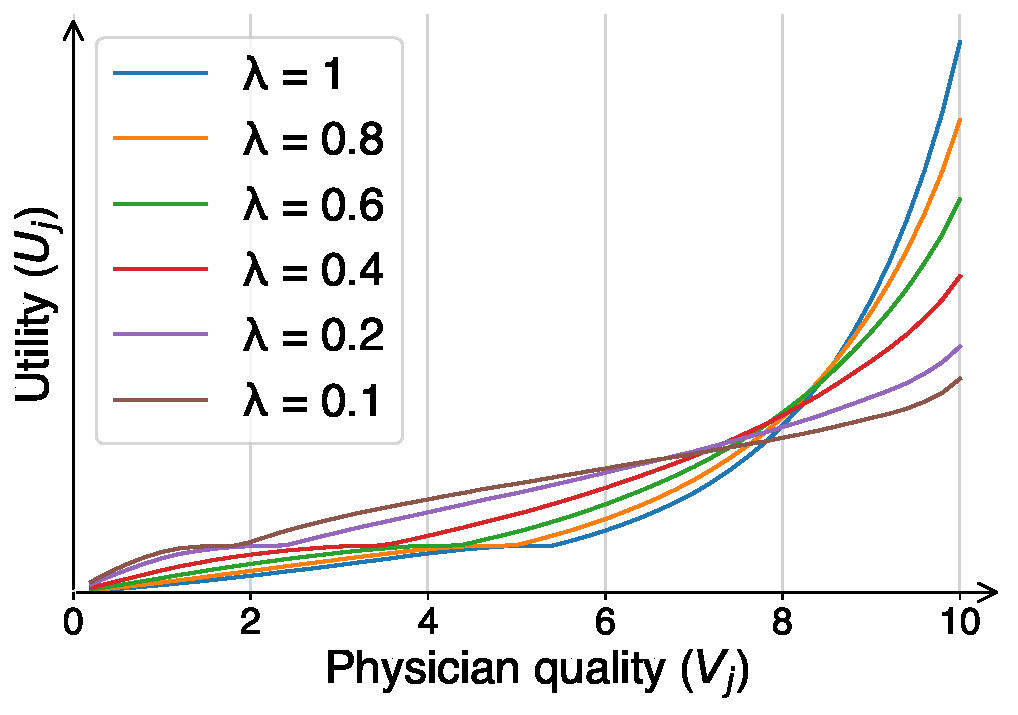
\includegraphics[width=\linewidth]{U.pdf}
        \vspace{-0.6cm}
        \caption{Logit model}
        \label{fig:logit_U}
    \end{subfigure}
    \hspace{0.05\linewidth}  % Space between the subfigures
    % Second subfigure
    \begin{subfigure}[b]{0.46\linewidth}
        \centering
        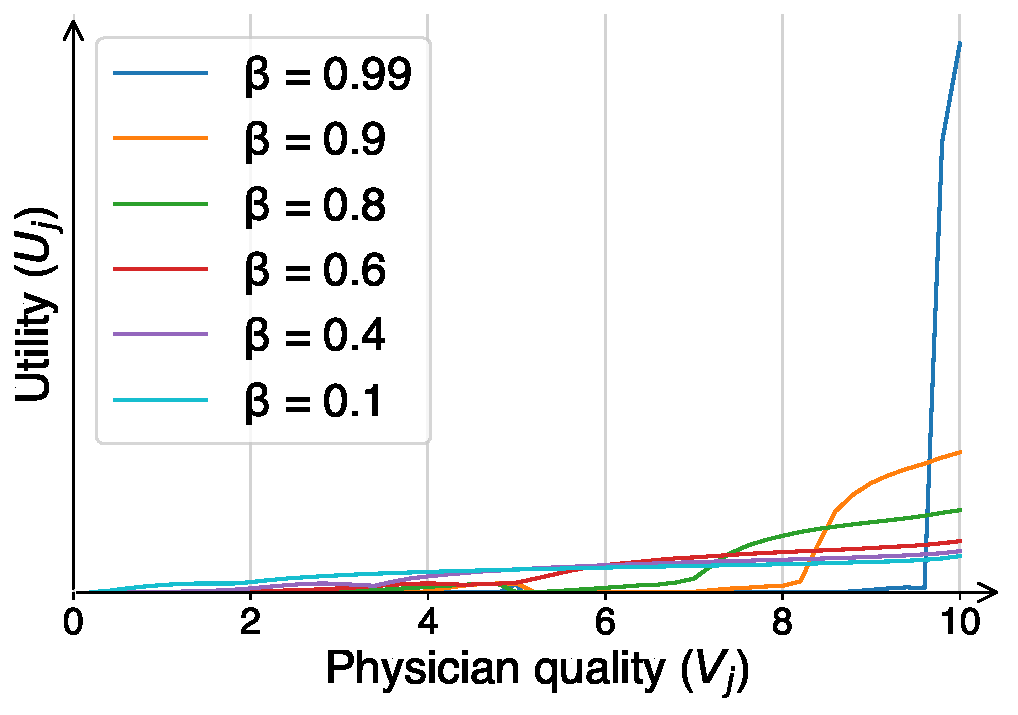
\includegraphics[width=\linewidth]{schnell_U.pdf}
        \vspace{-0.6cm}
        \caption{Sequential model}
        \label{fig:schnell_U}
    \end{subfigure}
    \caption{Equilibrium physician utility ($U_j$) by quality ($V_j$) \\ for different model parameters, equilibrium $\bar{\kappa}^*$}
    \label{fig:physician_U}
\end{figure}

\vspace{-0.25cm}

\begin{figure}[H]
    \centering
    % First subfigure
    \begin{subfigure}[b]{0.46\linewidth}
        \centering
        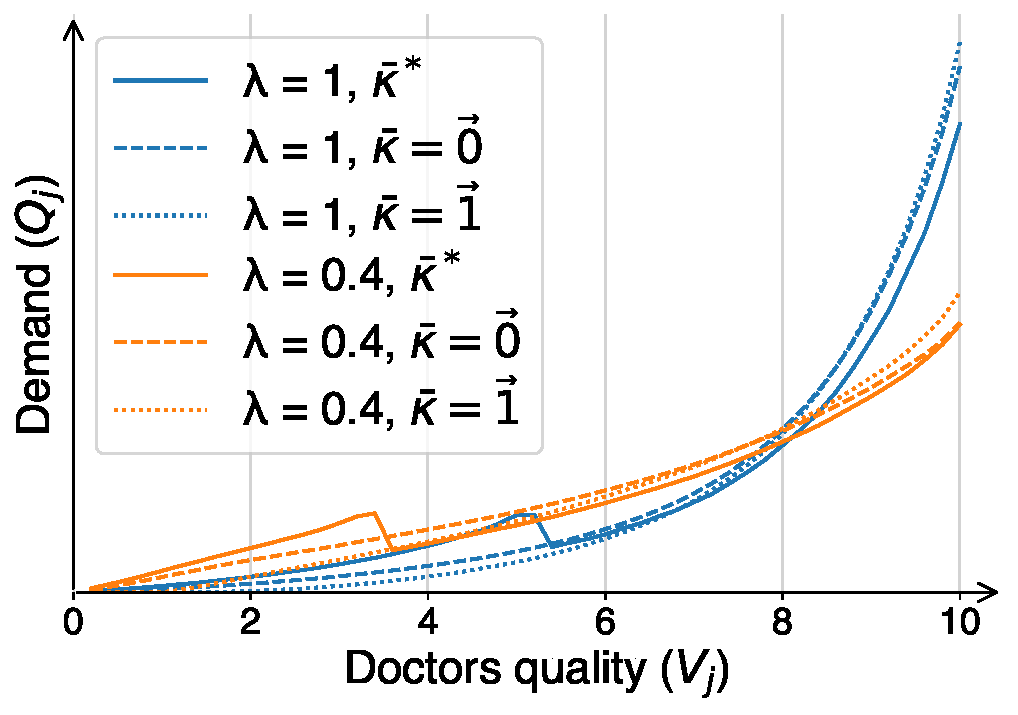
\includegraphics[width=\linewidth]{Q_comparison.pdf}
        \vspace{-0.6cm}
        \caption{Logit model}
        \label{fig:logit_Q_comp}
    \end{subfigure}
    \hspace{0.05\linewidth}  % Space between the subfigures
    % Second subfigure
    \begin{subfigure}[b]{0.46\linewidth}
        \centering
        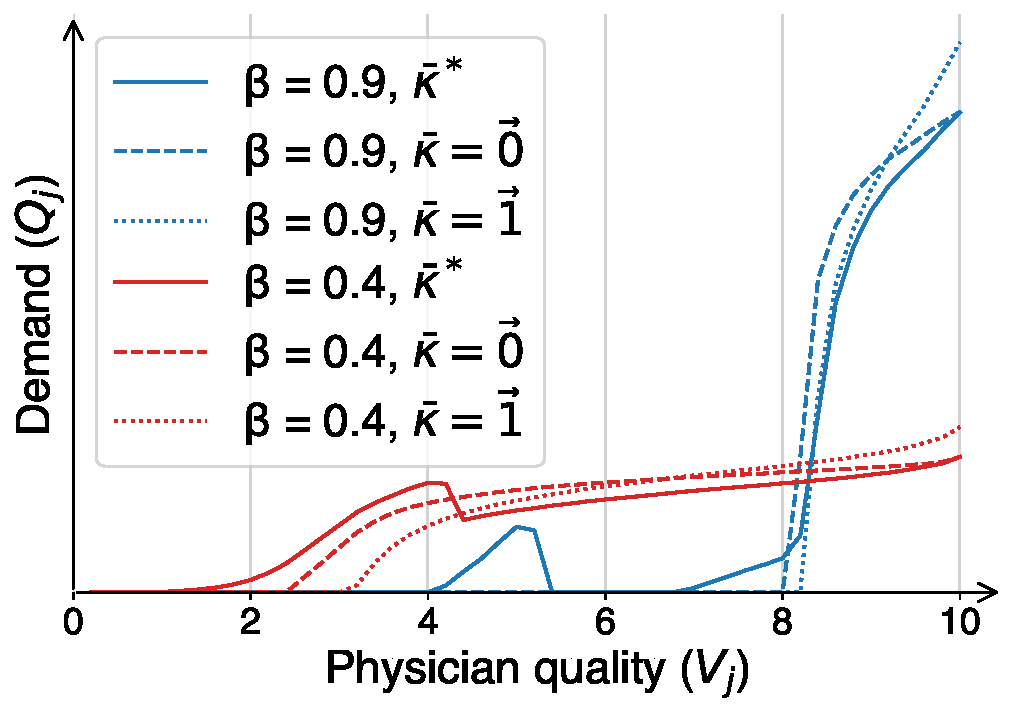
\includegraphics[width=\linewidth]{schnell_Q_comparison.pdf}
        \vspace{-0.6cm}
        \caption{Sequential model}
        \label{fig:schnell_Q_comp}
    \end{subfigure}
    \caption{Comparison of patient demand ($Q_j$) by physician quality ($V_j$)\\ for different model parameters and threshold vectors $\bar{\kappa}$}
    \label{fig:Q_comparison}
\end{figure}

\vspace{-0.25cm}

\begin{figure}[H]
    \centering
    % First subfigure
    \begin{subfigure}[b]{0.46\linewidth}
        \centering
        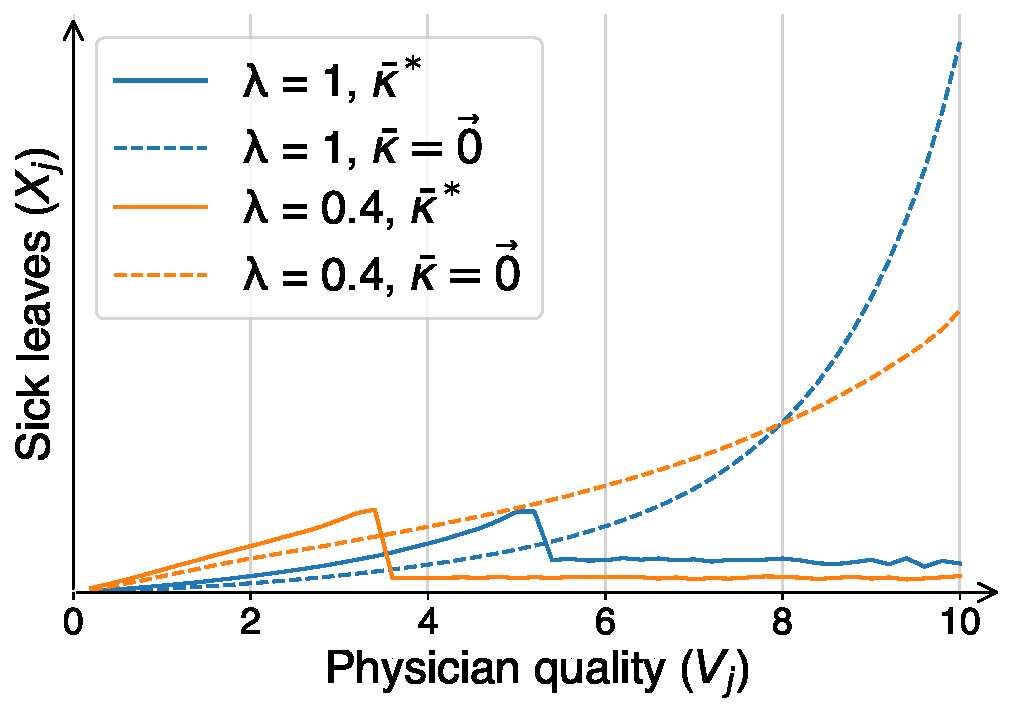
\includegraphics[width=\linewidth]{X_comparison.pdf}
        \vspace{-0.6cm}
        \caption{Logit model}
        \label{fig:logit_X_comp}
    \end{subfigure}
    \hspace{0.05\linewidth}  % Space between the subfigures
    % Second subfigure
    \begin{subfigure}[b]{0.46\linewidth}
        \centering
        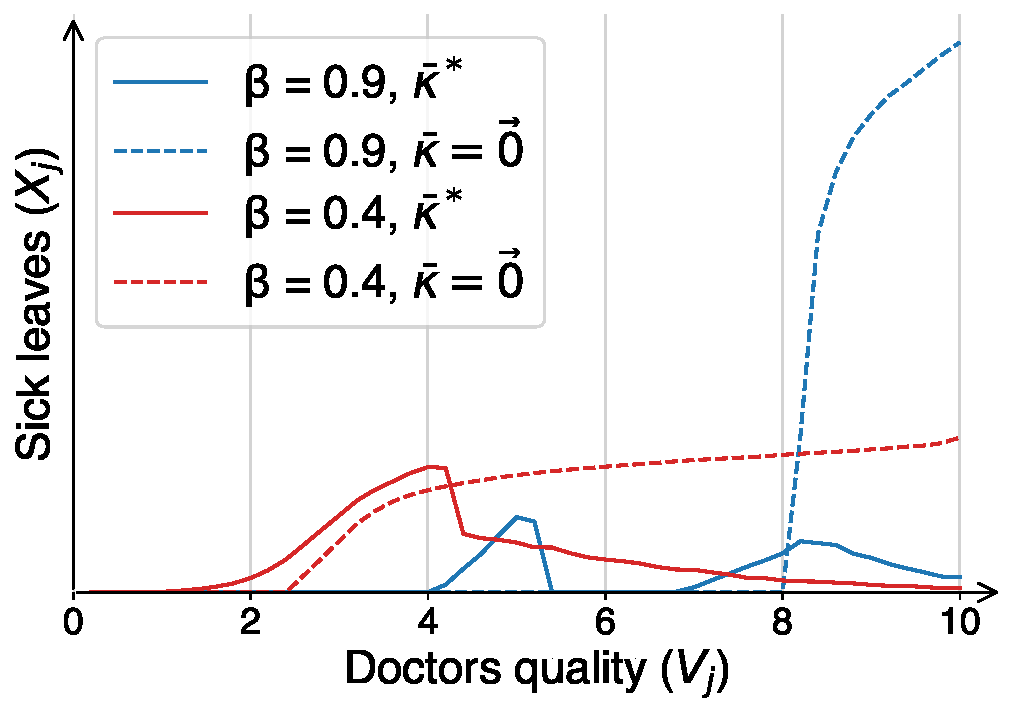
\includegraphics[width=\linewidth]{schnell_X_comparison.pdf}
        \vspace{-0.6cm}
        \caption{Sequential model}
        \label{fig:schnell_X_comp}
    \end{subfigure}
    \caption{Comparison of sick leaves issued ($X_j$) by physician quality ($V_j$)\\ for different model parameters and threshold vectors $\bar{\kappa}$}
    \label{fig:X_comparison}
\end{figure}

\newpage

\subsection{Identification Panels}
\label{sec:id}


\begin{figure}[H]
    \centering
    % First subfigure

    \begin{subfigure}[b]{0.39\linewidth}
        \centering
        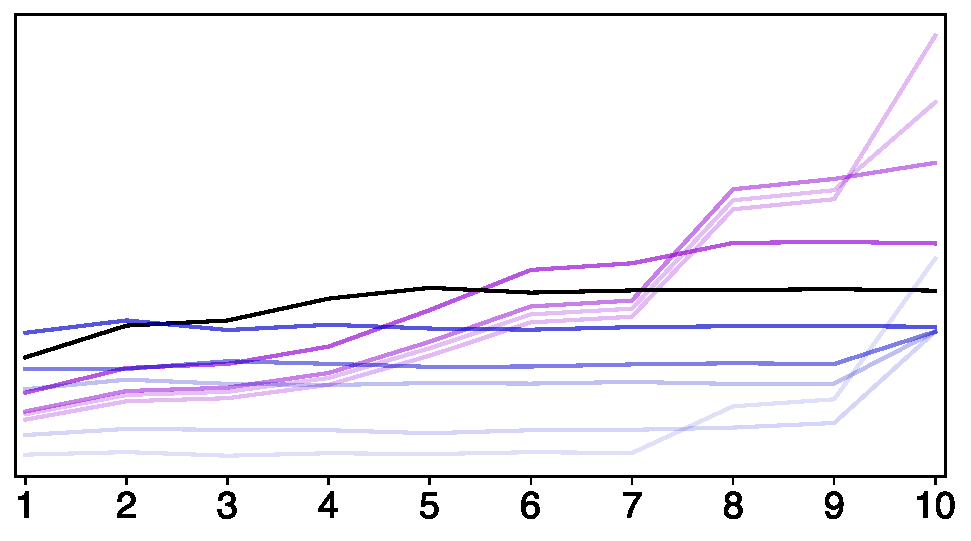
\includegraphics[width=\linewidth]{p_id1.pdf}
        \vspace{-0.6cm}
        \caption{$X_j$, variations in $p$}
        \label{fig:p1}
    \end{subfigure}
    \hspace{0.07\linewidth}  % Space between the subfigures
    % Second subfigure
    \begin{subfigure}[b]{0.39\linewidth}
        \centering
        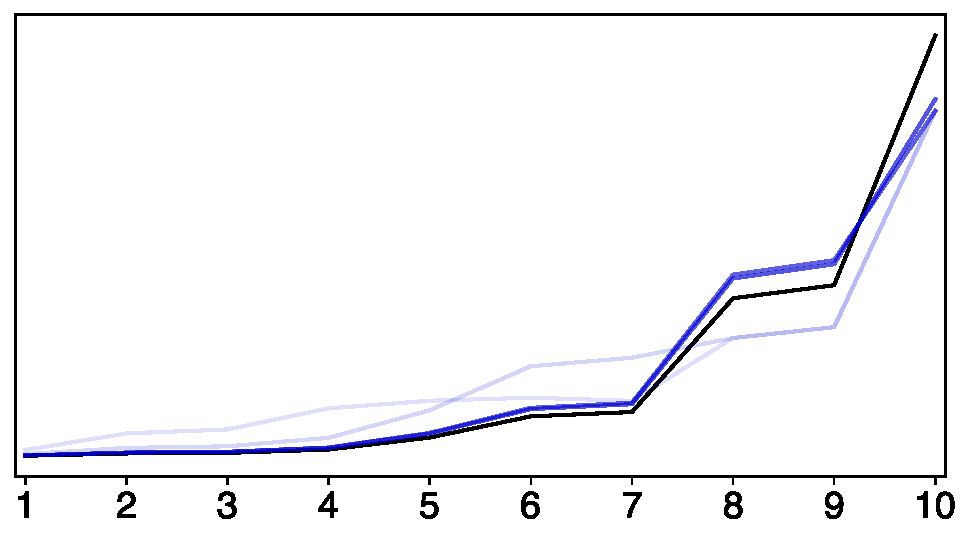
\includegraphics[width=\linewidth]{p_id2.pdf}
        \vspace{-0.6cm}
        \caption{$X_j^{30}$, variations in $p$}
        \label{fig:p2}
    \end{subfigure}

    \vspace{0.3cm}

    \begin{subfigure}[b]{0.39\linewidth}
        \centering
        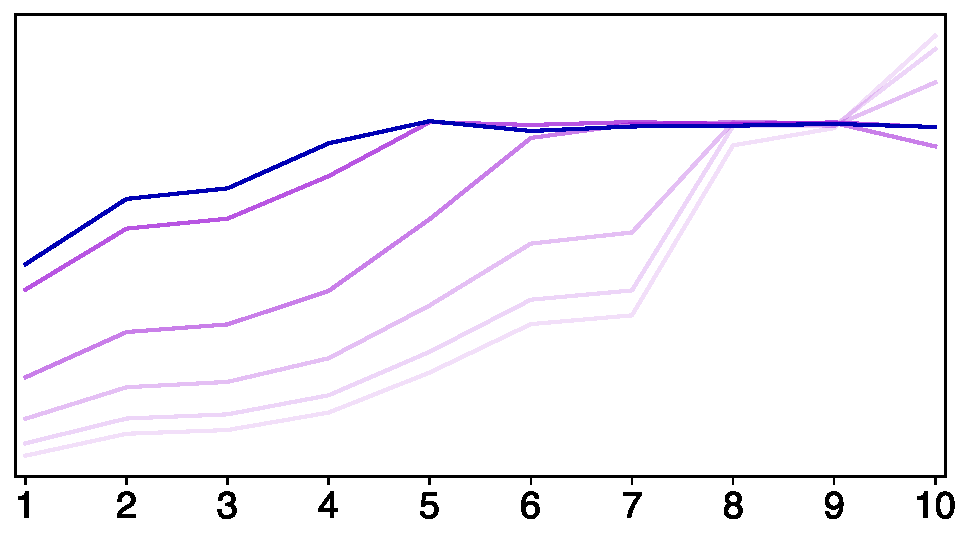
\includegraphics[width=\linewidth]{mu_id1.pdf}
        \vspace{-0.6cm}
        \caption{$X_j$, variations in $\mu$}
        \label{fig:mu1}
    \end{subfigure}
    \hspace{0.07\linewidth}  % Space between the subfigures
    % Second subfigure
    \begin{subfigure}[b]{0.39\linewidth}
        \centering
        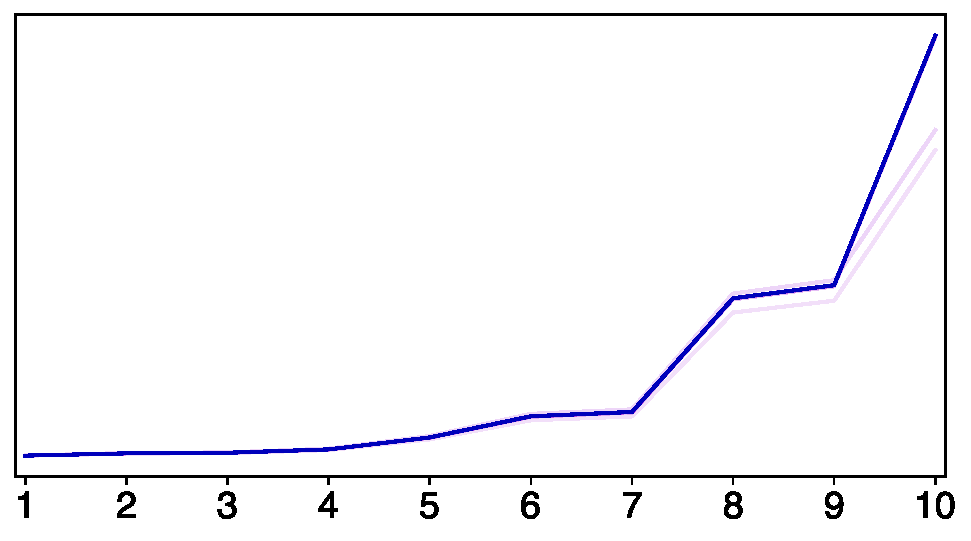
\includegraphics[width=\linewidth]{mu_id2.pdf}
        \vspace{-0.6cm}
        \caption{$X_j^{30}$, variations in $\mu$}
        \label{fig:mu2}
    \end{subfigure}

    \vspace{0.3cm}

    \begin{subfigure}[b]{0.39\linewidth}
        \centering
        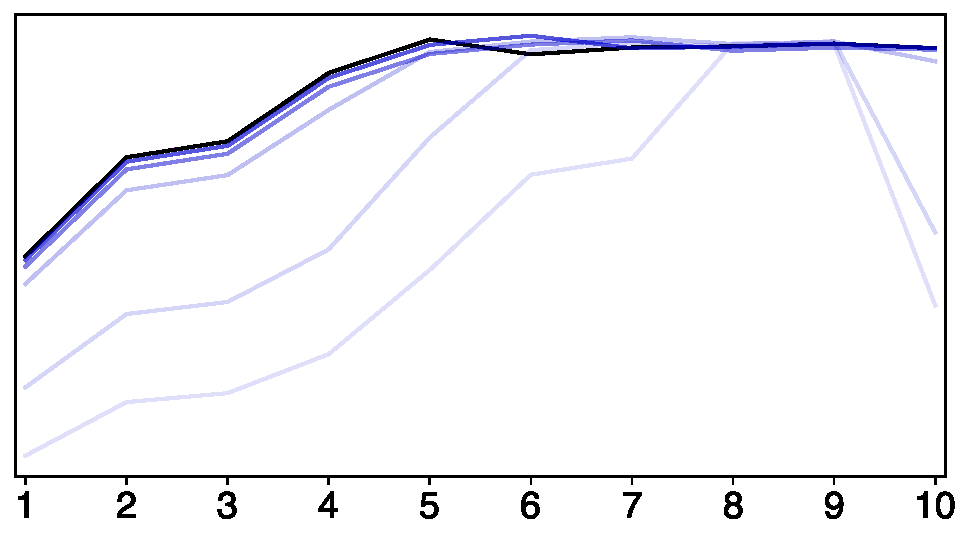
\includegraphics[width=\linewidth]{sigma_id1.pdf}
        \vspace{-0.6cm}
        \caption{$X_j$, variations in $\sigma$}
        \label{fig:sigma1}
    \end{subfigure}
    \hspace{0.07\linewidth}  % Space between the subfigures
    % Second subfigure
    \begin{subfigure}[b]{0.39\linewidth}
        \centering
        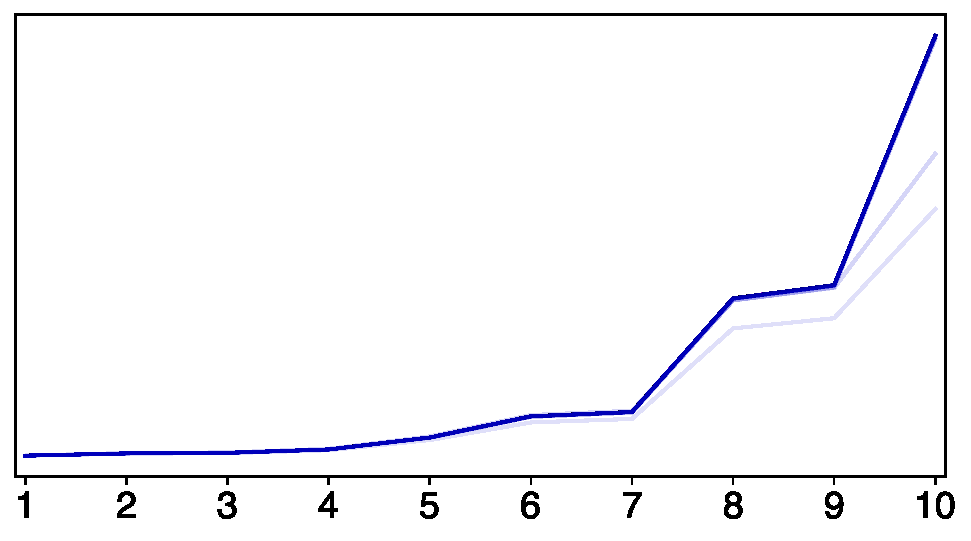
\includegraphics[width=\linewidth]{sigma_id2.pdf}
        \vspace{-0.6cm}
        \caption{$X_j^{30}$, variations in $\sigma$}
        \label{fig:sigma2}
    \end{subfigure}

    \vspace{0.3cm}

    \begin{subfigure}[b]{0.39\linewidth}
        \centering
        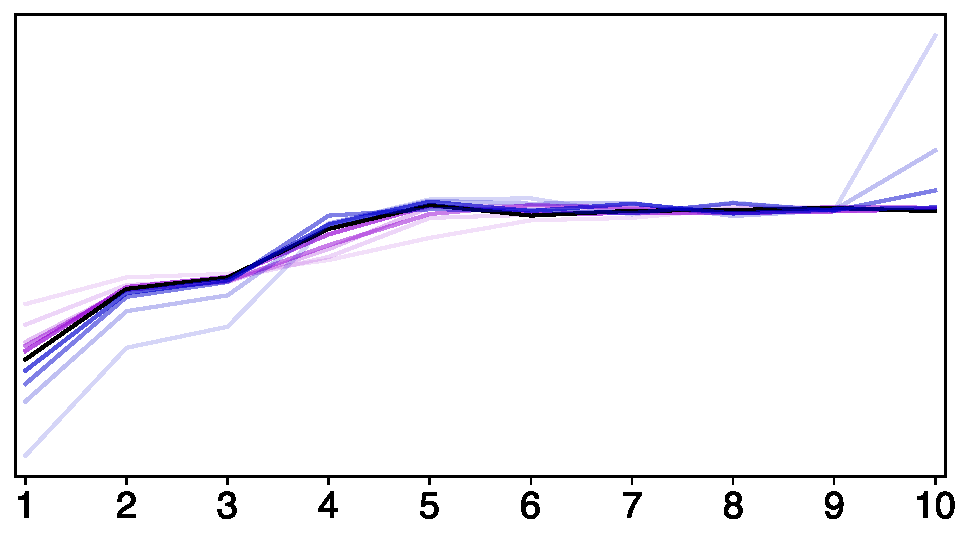
\includegraphics[width=\linewidth]{lambda_id1.pdf}
        \vspace{-0.6cm}
        \caption{$X_j$, variations in $\lambda_s$}
        \label{fig:lambda1}
    \end{subfigure}
    \hspace{0.07\linewidth}  % Space between the subfigures
    % Second subfigure
    \begin{subfigure}[b]{0.39\linewidth}
        \centering
        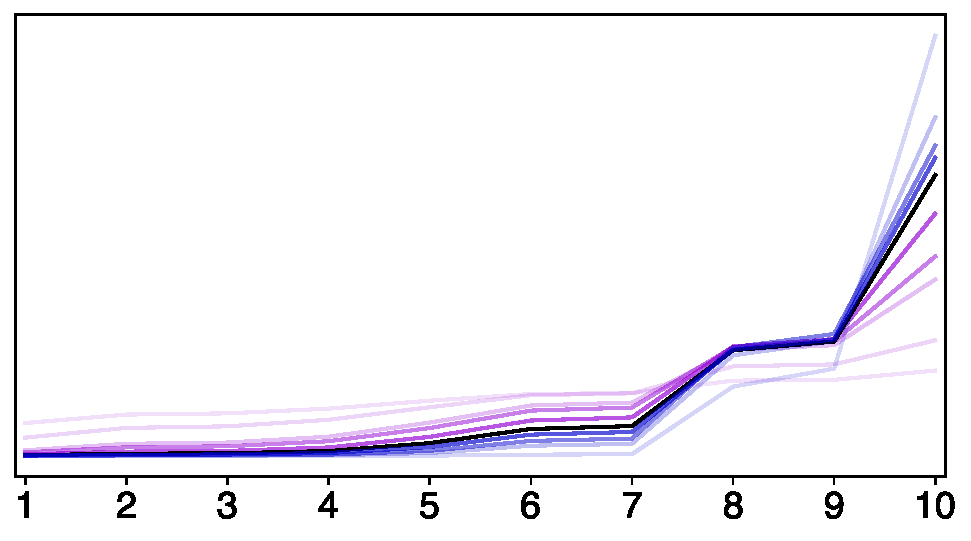
\includegraphics[width=\linewidth]{lambda_id2.pdf}
        \vspace{-0.6cm}
        \caption{$X_j^{30}$, variations in $\lambda_s$}
        \label{fig:lambda2}
    \end{subfigure}

    \vspace{0.3cm}

    \begin{subfigure}[b]{0.39\linewidth}
        \centering
        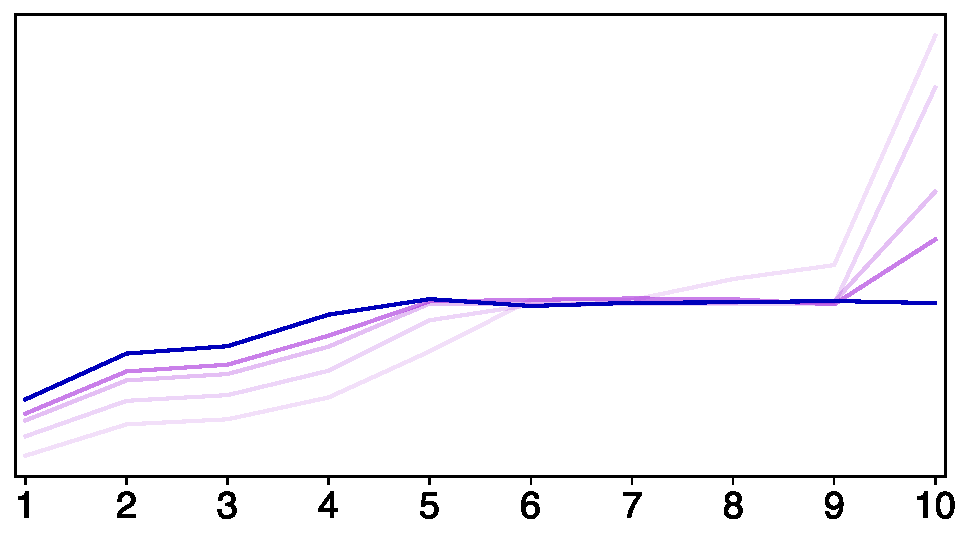
\includegraphics[width=\linewidth]{k_id1.pdf}
        \vspace{-0.6cm}
        \caption{$X_j$, variations in $\bar{\kappa}_{\max}$}
        \label{fig:k1}
    \end{subfigure}
    \hspace{0.07\linewidth}  % Space between the subfigures
    % Second subfigure
    \begin{subfigure}[b]{0.39\linewidth}
        \centering
        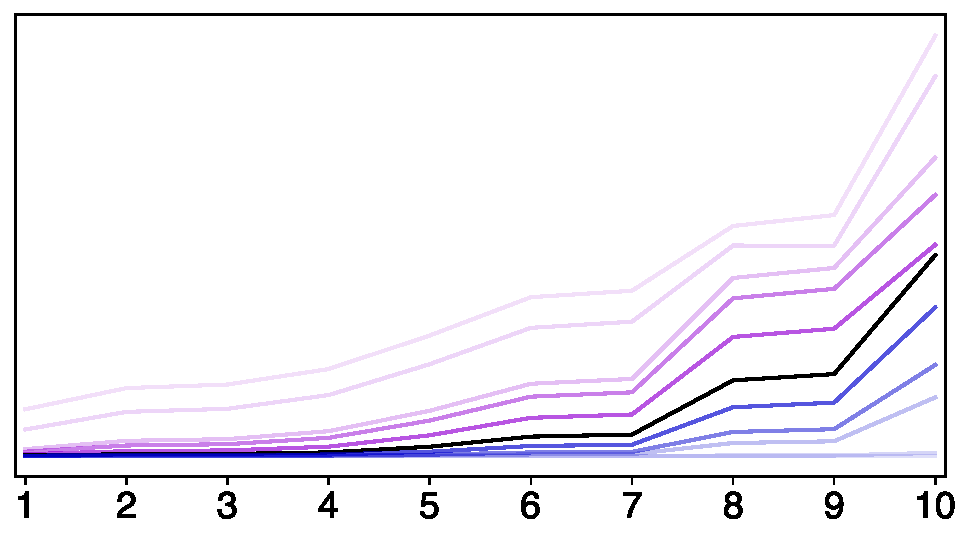
\includegraphics[width=\linewidth]{k_id2.pdf}
        \vspace{-0.6cm}
        \caption{$X_j^{30}$, variations in $\bar{\kappa}_{\max}$}
        \label{fig:k2}
    \end{subfigure}


\caption{Sick leaves issued by quality bin as parameters vary.}
\label{fig:identification}
\vspace{0.2em}
{\small Black: Estimated value. Violet: Lower. Blue: Higher.
\vspace{-0.2em}

Transparency increasing with distance from estimated value}


\end{figure}


\subsection{Parameter Sources}
\label{sec:par}

\subsubsection*{Physician quality by bins ($V_1$ ... $V_{10}$)}

As mentioned in the main text, three criteria are considered for the \textit{quality score}:
\begin{enumerate}[label=\roman*, itemsep=0pt, topsep=0pt]
    \item Average duration of sick leaves issued.
    \item Percentage of sick leaves of 30+ days over total in sampled period.
    \item Amount of sick leaves of 30+ days issued.
\end{enumerate}

For each of the criteria the \textit{percentile rank} which each physician occupies is recorded, all in increasing order, i.e. from lowest to highest average duration, from lowest to highest percentage/amount of $\geq30$ days sick leaves. Call the percentile rank which physician $j$ occupies in each category $p_j^{i}$, $p_j^{ii}$ and $p_j^{iii}$. The \textit{quality score} of physician $j$ is the simple average of these three, that is:
\[
q\_score_j \;=\; \frac{1}{3}p_j^{i} \;+\; \frac{1}{3}p_j^{ii} \;+\; \frac{1}{3}p_j^{iii}
\]

The quality bins are then set up from the decile ranks of physicians in their \textit{quality score}. Bin 1, for example, is simply the first decile rank of $q\_score$, the lowest 10\% of physicians according to their quality score. Each bin is therefore equally sized.

The parameters $V_1$ ... $V_{10}$ associated with each bin are then to be estimated in our GMM exercise, subject to the constraint that they increase in alignment with quality. Simply put: $ V_{10} > V_{9} > ... > V_{1}$.

\subsubsection*{Revenue by visit ($r_j$) and cost of visit ($\tau_j$)}

We use a single $r$ and $\tau$ for all physicians on this occasion. In the future a proper match to revenue bins would be a way to further square parameter estimation. Our procedure is arbitrary, but an alternative method would nonetheless stay within the same degree of magnitude as our final values for $r$ and $\tau$, so in this case arbitrariness is not all too relevant.

We select the ten most frequent $cie10$ categories in our sample, the international standard classification of medical conditions. These ten, as well as non-categorized conditions (seen as \textit{empty} in the Table), account for 47.91\% of all sick leaves in our database. We then match the conditions to a particular field of practice, though strictly speaking physicians aren't reduced to their own field when issuing sick leaves, so matching is fuzzy.

We then take a \textit{full price} and the {fee} paid by FONASA affiliates in the Free Choice Modality (MLE) as a reference price, from a tariff book assembled by FONASA itself (\citeyear{fonasa}). We take this to correspond to the physician's revenue by visit ($r$) and the patients' cost of visit ($\tau$), respectively.

Our final value for $r$ and $\tau$ is the weighted average of this prices, weighted by the relative frequency of each category and its matched full and benefit price. This amounts to taking the dot product of the `\%' column with the `Full Price' and `Aff. Fee' columns in the Table below, respectively.

The resulting values are: $r = 21,182$ and $\tau = 8,944$. For simplicity, we select to use them in the thousands for estimation, i.e. 8.944 instead of 8,944. See the Table below for the referenced variable columns.

\begin{table}[H]
    \centering
\footnotesize
    \begin{tabular}{lrrllrr}
    \toprule
    \textit{cie10} cat. & Instances & \% & Informal Description & Matched Field & Full Price & Aff. Fee  \\
    \midrule
    M54            & 379,332    & 0.20       & Back pain            & Traumatology  & \$ 18,130 & \$ 7,250    \\
    F32            & 304,399    & 0.16       & Depression           & Psychiatry    & \$ 27,510 & \$ 11,000  \\
    F41            & 284,129    & 0.15       & Anxiety              & Psychiatry    & \$ 27,510 & \$ 11,000   \\
    F43            & 244,468    & 0.13       & Stress               & Psychiatry    & \$ 27,510 & \$ 11,000   \\
    J20            & 191,615    & 0.10       & Bronchitis           & General       & \$ 14,270 & \$ 7,440    \\
    A09            & 186,535    & 0.10       & Gastroenteritis      & General       & \$ 14,270 & \$ 7,440    \\
    \textit{empty}  & 152,239   &            &                      &               &       &         \\
    M75            & 115,585    & 0.06       & Shoulder             & Traumatology  & \$ 18,130 & \$ 7,250   \\
    J00            & 92,660     & 0.05       & Common cold          & General       & \$ 14,270 & \$ 7,440    \\
    M51            & 54,800     & 0.03       & Intervertrebal disc  & Traumatology  & \$ 18,130 & \$ 7,250    \\
    K52            & 49,182     & 0.03       & Gastroenteritis      & General       & \$ 14,270 & \$ 7,440    \\
    \bottomrule
    \end{tabular}
    \caption{Most common health conditions reported by physicians in sick leaves issued, matched to corresponding fees of service}
    \label{tab:cond}
\end{table}

\end{document}
